\documentclass[11pt]{article}
\usepackage{geometry}                % See geometry.pdf to learn the layout options. There are lots.
\geometry{letterpaper}                   % ... or a4paper or a5paper or ... 
%\geometry{landscape}                % Activate for for rotated page geometry
%\usepackage[parfill]{parskip}    % Activate to begin paragraphs with an empty line rather than an indent
\usepackage{graphicx}
\usepackage{amssymb}
\usepackage{amsmath}
\usepackage{epstopdf}
\usepackage{hyperref}
\DeclareGraphicsRule{.tif}{png}{.png}{`convert #1 `dirname #1`/`basename #1 .tif`.png}


\graphicspath{
{/Users/Andy/Springboard_DataScience/Capstone_1/figures/}
}

\title{Capstone 1 Milestone Report - Analyzing NYC Citibke Usage}
\author{Andy Pickering}
%\date{}                                           % Activate to display a given date or no date



\begin{document}
\maketitle

\tableofcontents
\newpage


%~~~~~~~~~~~~~~~~~~~~~
\section{Introduction}

For my first capstone project, I chose to analyze data from the NYC Citibike bike-rental system.
The problem is to develop a model to predict the number of rides taken each day on the Citibike system. The main client is the Citibike management, who need to plan for anticipated demand and ensure that there are enough working bikes and staff on hand to meet the demand. Other clients could include city transportation departments, since bike usage likely affects ridership on other modes of transportation, as well as possibly introducing traffic issues. A more ambitious goal is to predict bike demand and availability at specific stations, to determine the most efficient distribution of bikes. 




%~~~~~~~~~~~~~~~~~~~~~~~~~~~~~~~~~~~~~~
\section{Data}



\subsection{Historical Data}
The main dataset is historical records of trips taken on the Citibike system. These are made available by the Citibike program at \url{https://www.citibikenyc.com/system-data} in monthly files, spanning the time range July 2013 to March 2017. Each row in the dataset corresponds to one ride, and includes the following fields:

\begin{itemize}
\item Trip Duration (seconds)
\item Start Time and Date
\item Stop Time and Date
\item Start Station Name
\item End Station Name
\item Station ID
\item Station Lat/Long
\item Bike ID
\item User Type (Customer = 24-hour pass or 7-day pass user; Subscriber = Annual Member)
\item Gender (Zero=unknown; 1=male; 2=female)
\item Year of Birth
\end{itemize}

Station-related variables except id (name, lat,long ) are not saved in the table with ride data, in order to reduce the size. A separate table 'stations' is made with the info for unique stations, which can be joined to the 'rides' table using the station ID key if needed.

Upon examining the rider age distribution, there appear to be a small number of incorrect values or typos. A very small fraction of riders have ages over 100, up to 159!. Since the oldest living person is 116 it seems likely that these are mistakes in the data. Birth year, not age, was recorded, so my best guess is that 18 was intered instead of 19 for the beginning of some years (ie 1895 instead of 1995). These age values will be converted to NaN in the dataset.




\subsection{Weather}

Historical daily weather data was downloaded from the Weather Underground website (\url{www.wunderground.com}) with the script \verb+get_weather_data.py+ . I use data from LaGuardia airport. The data contains the following fields:

\begin{itemize}
\item Max Temperature (F)
\item Min Temperature (F)
\item Mean Temperature (F)
\item Precipitation (inches)
\item Events (rain,snow,fog etc.)
\item Cloud cover
\item Max wind gust (mph)
\end{itemize}


\subsection{Holidays}

A list of US holidays was obtained through the holiday API. \url{https://holidayapi.com/}. This contains the name of each holiday and the date observed.


\subsection{Limitations}

Historical citibike data does not include any user ID, so I cannot determine the number of unique users or individual patterns.

Historical data does not include station status (number of bikes available etc). So I cannot predict station availability from this data. I began collecting streaming data in order to address this question in the future.




%~~~~~~~~~~~~~~~~~~~~~~~~~~~~~~~~~~~~~~
\section{Data cleaning and wrangling}

A deeper dive into the data set:
What important fields and information does the data set have?
What are its limitations i.e. what are some questions that you cannot answer with this data set?
What kind of cleaning and wrangling did you need to do?
Are there other datasets you can find, use and combine with, to answer the questions that matter?

The combined historical citibike data was very big; therefore I decided to store the data in a sqlite3 database and then query the database from python for analysis. A python script (\verb+read_citibike_to_sql.+) was used to perform some cleaning and modification of the data and write it to the database. Cleaning/modifications performed on the historical data include:

\begin{itemize}
\item Replacing spaces in variable names w/ underscores
\item Converting date fields to appropriate data types
\item Add variables such as year,month, and day to the dataframe
\item Converting variables x,x to categorical data type
\end{itemize}





%~~~~~~~~~~~~~~~~~~~~~~~~~~~~~~~~~~~~~~
\section{Analysis}

Any preliminary exploration you�ve performed and your initial findings. Test the hypotheses one at a time. Often, the data story emerges as a result of a sequence of testing hypothesis e.g. You first tested if X was true, and because it wasn't, you tried Y, which turned out to be true.


\subsection{Citibike Usage}

I began with an exploratory analysis of the data and patterns of ridership.

Findings:

\begin{itemize}

\item Ridership has increased over the 3 years (Figure \ref{rides_vs_year}).

\item  Part of this increase is due to expanasions of the system, increasing the number of stations and bikes. (Figure \ref{rides_vs_stations}). I computed the number of stations each month as the number of unique station IDs in all the rides during that time. Note this only includes stations that were actually used; I assume every available station was used at least once, although the actual number of stations could be slightly different. I think it is close enough to account for the majority of this effect though.

\item There is a strong seasonal cycle during each year, with more rides in the summer and early fall. (Figure \ref{rides_vs_month_eachyear}). My assumption is that a lot of this is due to the seasonal cycle in weather; this will be tested further.

\item Daily cycle: During the week, the majority of rides take place during the morning and evening rush hours (Figure \ref{rides_vs_hr_wkday}). On the weekend, rides are more distributed throughout the day (Figure \ref{rides_vs_hr_wkend}).

\item A quick map examination of the most used stations showed that during the week, there are several stations close to mass transit such as Grand Central Stations?. On weekends, those stations are not most used; and several of the most used stations are now located near Central Park. This adds further evidence to the pattern of commuting during the week and recreational riding on weekends.

\item The avearage duration of rides is longer on the weekend. A t-test found this difference is statistically significant.

\end{itemize}




\begin{figure}[htbp]
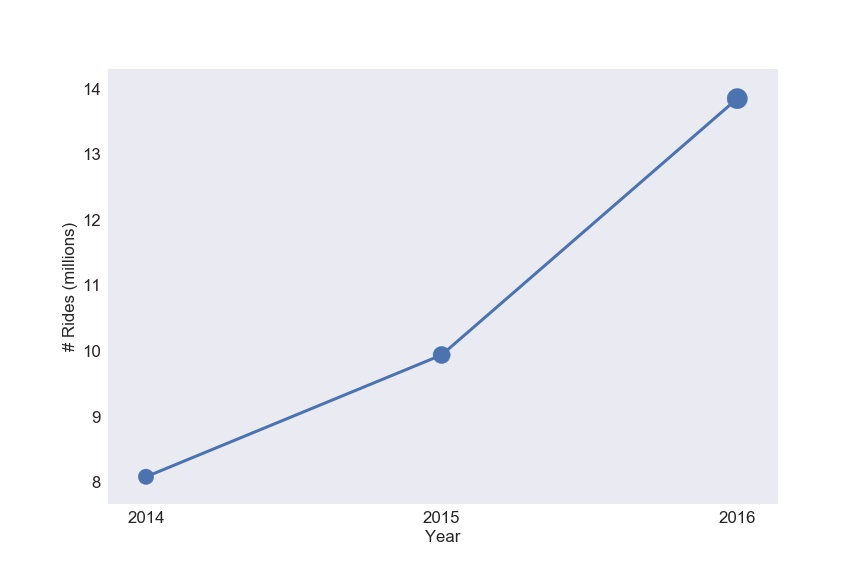
\includegraphics[width=40pc]{rides_per_year.jpg}
\caption{Total number of rides ( in millions) taken each year. Only years for which complete data was available are plotted.}
\label{rides_vs_year}
\end{figure}

\begin{figure}[htbp]
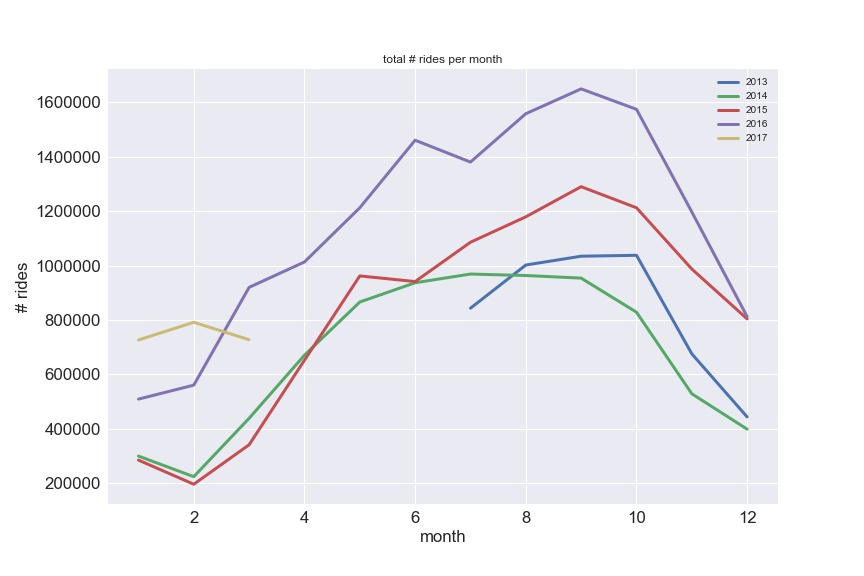
\includegraphics[width=40pc]{rides_per_month_each_year.jpg}
\caption{Total number of rides taken each month, for different years.}
\label{rides_vs_month_eachyear}
\end{figure}

\begin{figure}[htbp]
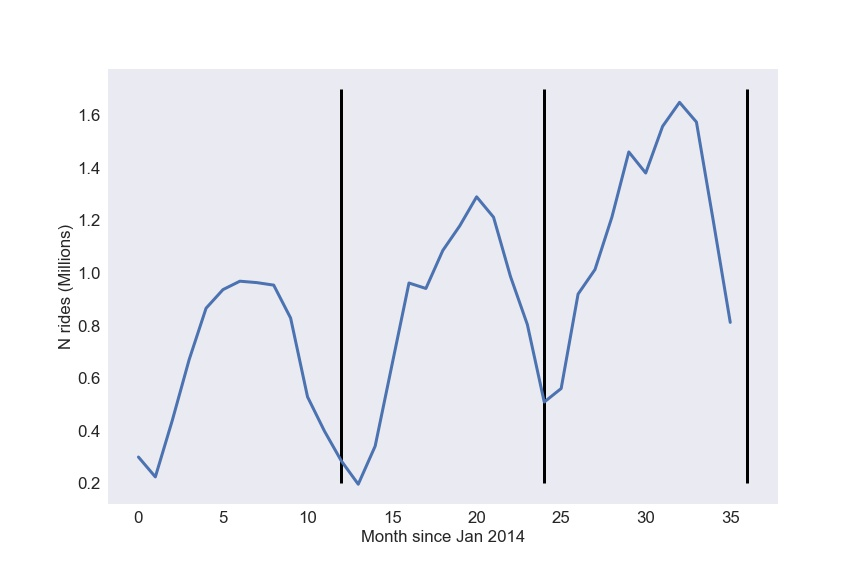
\includegraphics[width=40pc]{rides_per_month.jpg}
\caption{Total number of rides taken per month, plotted consecutively for 2014-2016.}
\label{rides_vs_month}
\end{figure}


% number of stations

\begin{figure}[htbp]
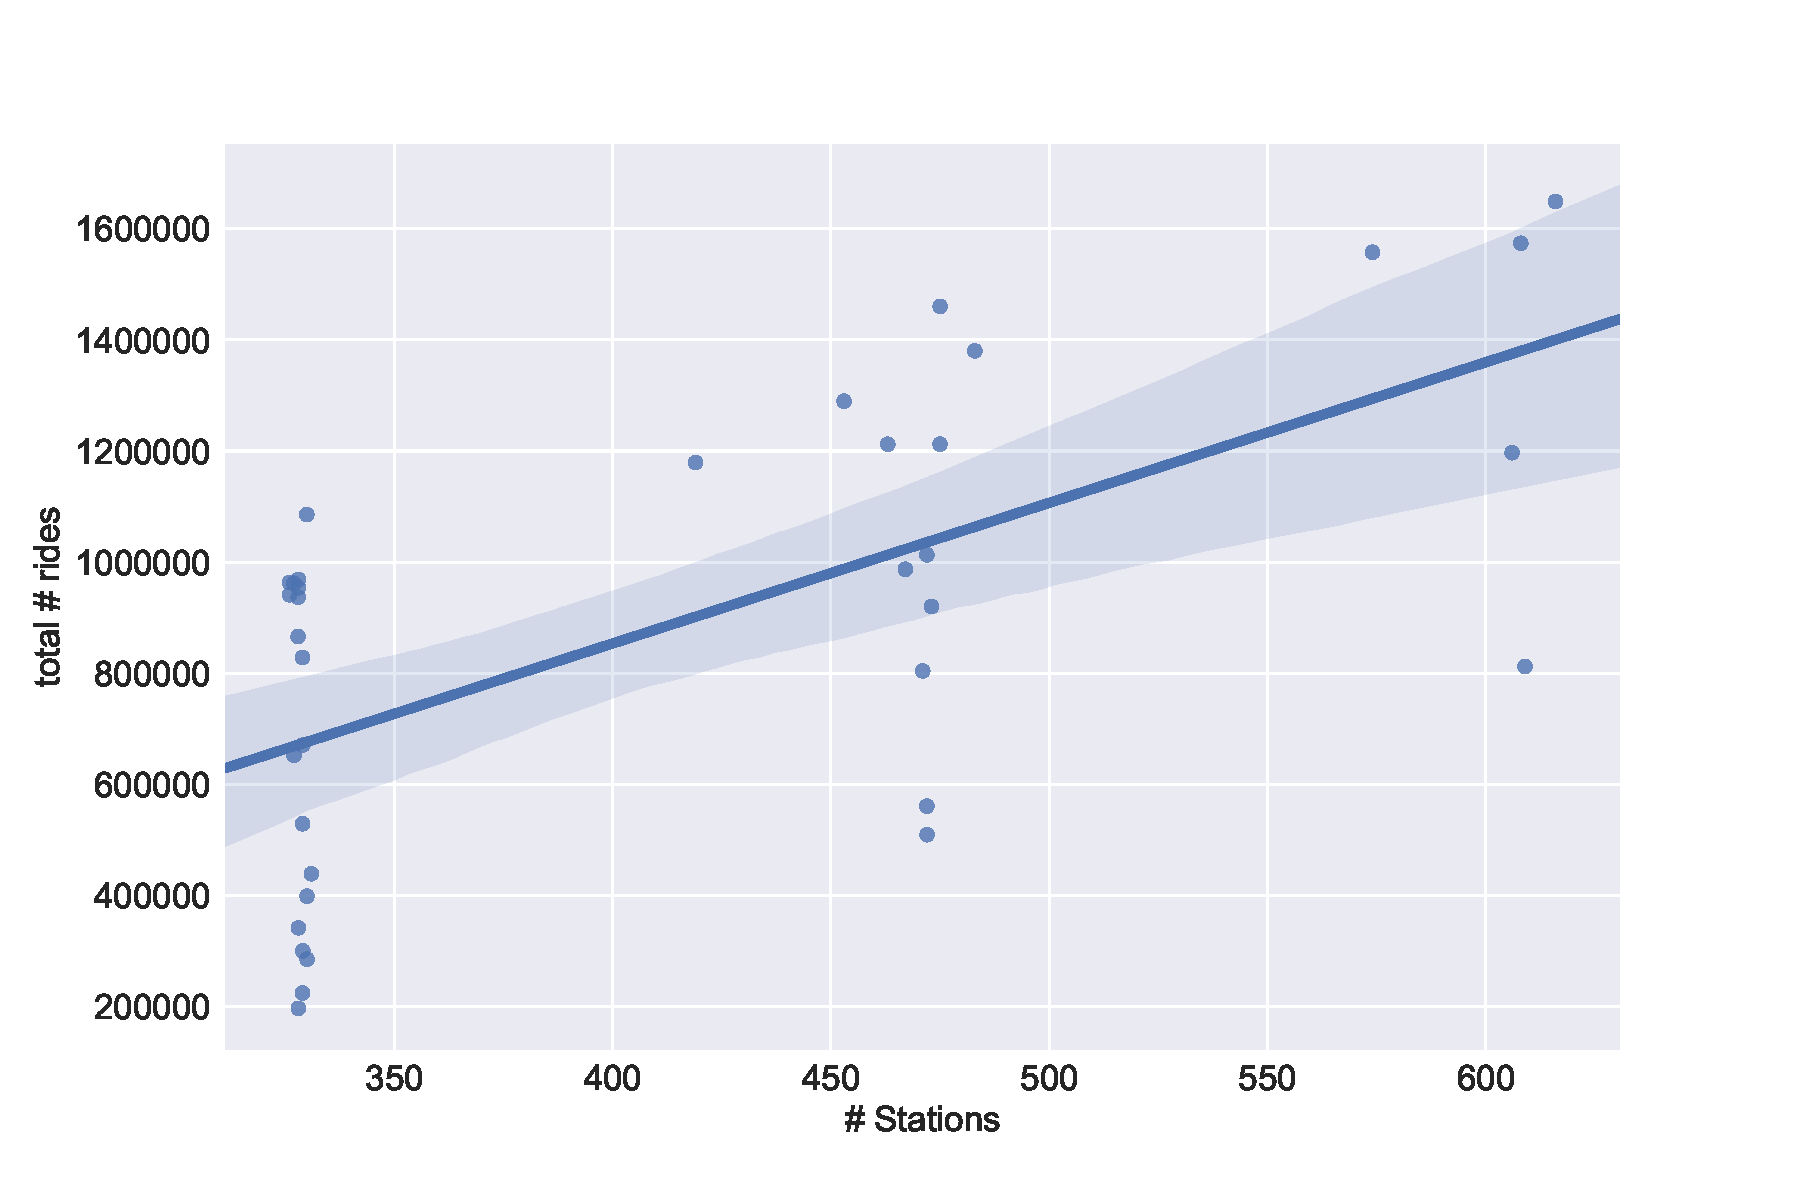
\includegraphics[width=40pc]{rides_vs_stations.pdf}
\caption{Total number of rides vs the number of stations.}
\label{rides_vs_stations}
\end{figure}




\begin{figure}[htbp]
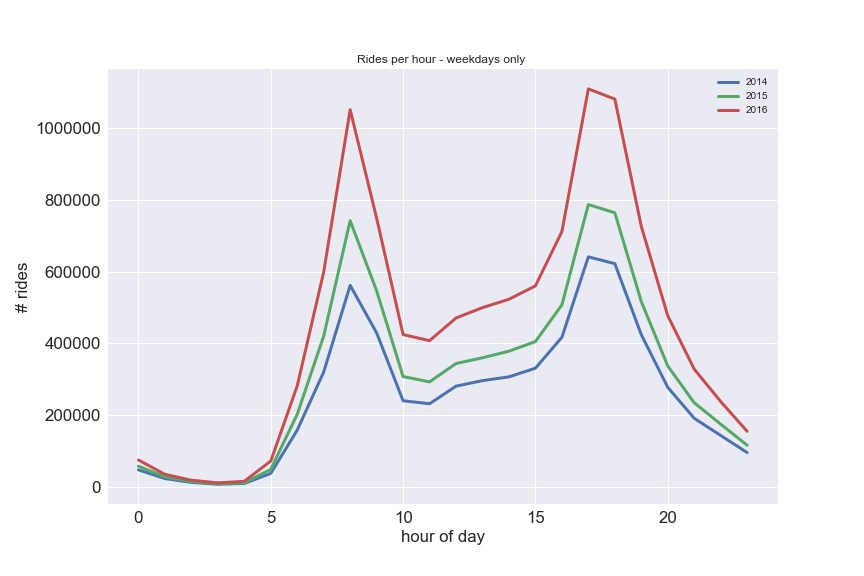
\includegraphics[width=40pc]{rides_per_hour_weekdays.jpg}
\caption{Total number of rides taken each hour of day, for weekdays (Monday-Friday).}
\label{rides_vs_hr_wkday}
\end{figure}

\begin{figure}[htbp]
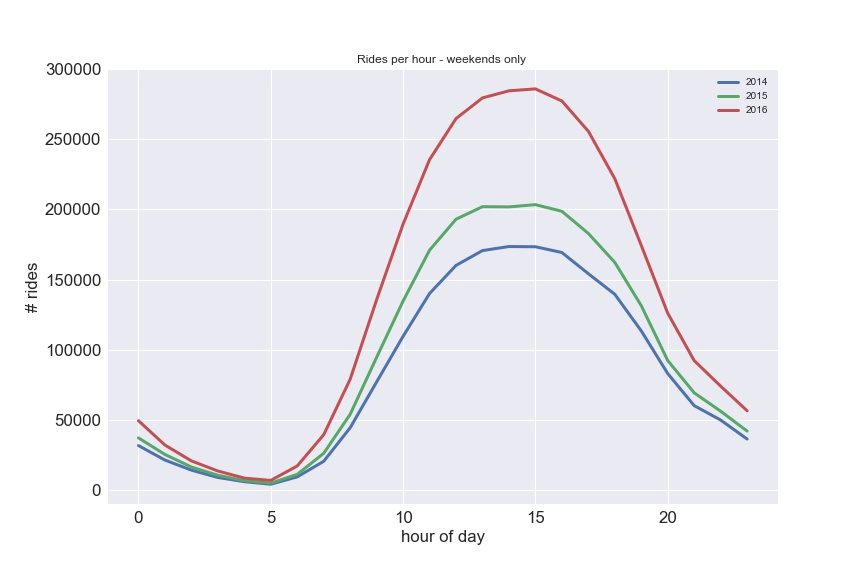
\includegraphics[width=40pc]{rides_per_hour_weekends.jpg}
\caption{Total number of rides taken each hour of day, for weekend days (Saturday and Sunday).}
\label{rides_vs_hr_wkend}
\end{figure}


\begin{figure}[h]
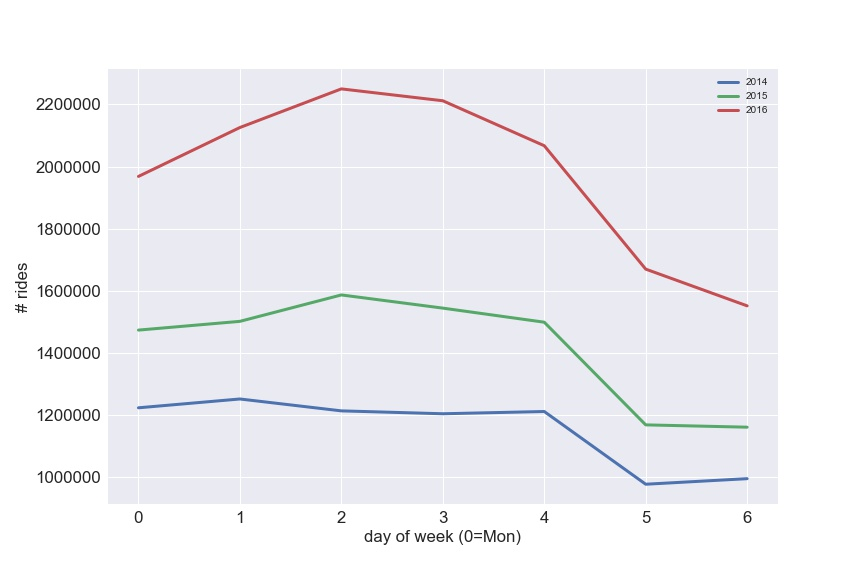
\includegraphics[width=40pc]{rides_per_weekday.jpg}
\caption{Total number of rides taken for each day of the week. Monday is day 0.}
\label{rides_vs_dyofwk}
\end{figure}



\subsection{Relationship with Weather}


The daily number of rides is postitively correlated with temperature (Figure \ref{rides_vs_temp}). This makes sense; anyone who has ridden a bike knows it is much more enjoyable when it's not freezing! A linear regression for 2015 data gives an $R^2$ of $0.62$. It appears that there is a lot more variance for temperatures above 50$^o$; this is something to look into further. I think this may be partly due to added stations in mid 2016.


\begin{figure}[h]
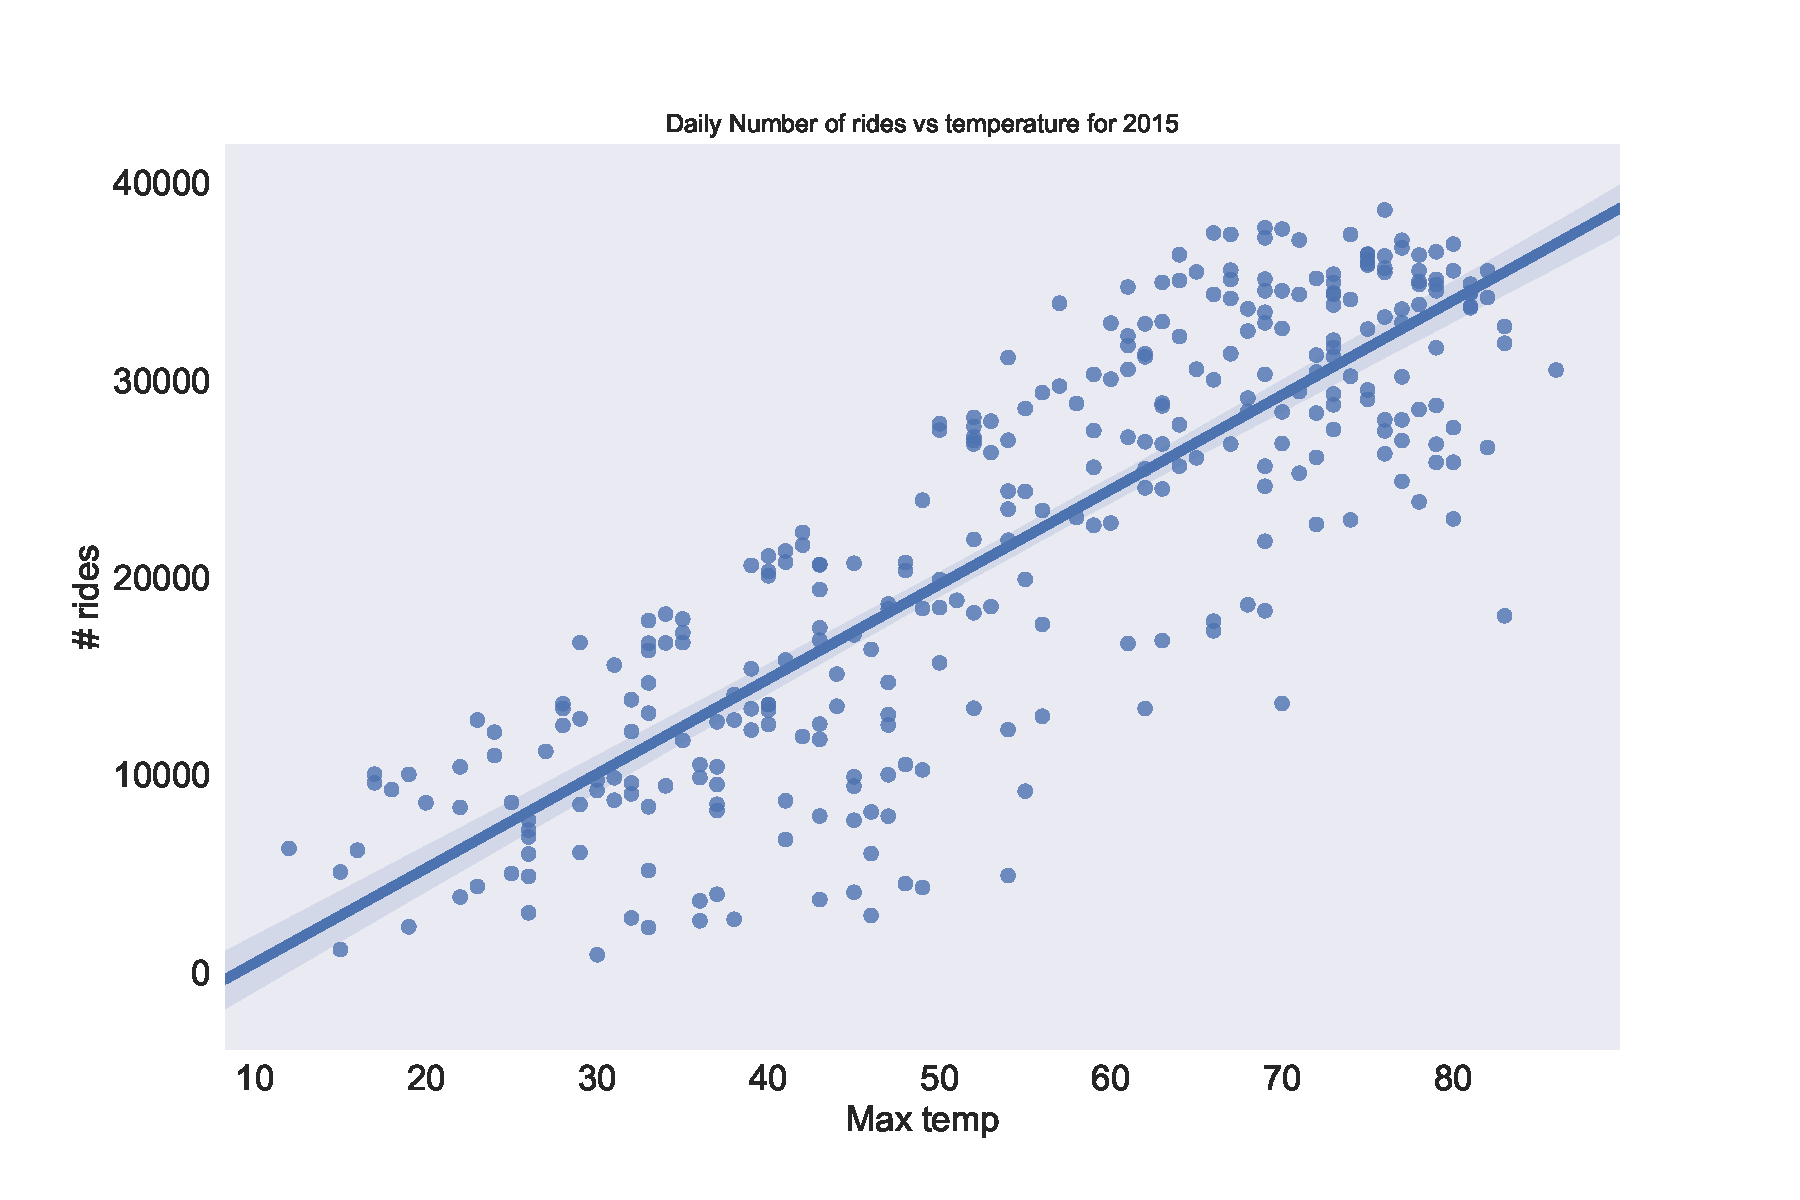
\includegraphics[width=40pc]{rides_vs_temp_2015.pdf}
\caption{Total number of rides vs temperature in 2015.}
\label{rides_vs_temp}
\end{figure}



%~~~~~~~~~~~~~~~~~~~~~~~~~~~~~~~~~~~~~~
\section{Regression Model}








%~~~~~~~~~~~~~~~~~~~~~~~~~~~~~~~~~~~~~~
\section{Conclusions and Plan}

At this point in the project, I have the following conclusions:

\begin{itemize}

\item There is a strong weekday/weekend pattern to the number of rides. More rides are taken during the week than on weekends. On weekdays, the majority of rides are taken during rush hours, suggesting heavy use of the system for commuting. On weekends, rides are more distributed throughout the day, suggesting more recreational use of the system. 

\item An important factor which I did not anticipate before doing the analysis is the changing number of stations and bikes, which essentially raises the baseline level of rides. This needs to be accounted for when trying to diagnose the effect of other variables such as temperature.

\item The number of rides is positvely correlated with the daily mean temperature. A linear regression 

\end{itemize}


Plan:

\begin{itemize}
\item Look at other weather variables such as rain, clouds, etc;
\item Build regression model to try to predict number of rides.
\item 
\end{itemize}



\end{document}  


